\documentclass[nojss]{jss}
\usepackage[sc]{mathpazo}
\usepackage{geometry}
\geometry{verbose,tmargin=2.5cm,bmargin=2.5cm,lmargin=2.5cm,rmargin=2.5cm}
\setcounter{secnumdepth}{2}
\setcounter{tocdepth}{2}
\usepackage{breakurl}
\usepackage{hyperref}
\usepackage[ruled, vlined]{algorithm2e}
\usepackage{mathtools}

\usepackage{float}
\usepackage{placeins}
\usepackage{mathrsfs}
\usepackage[toc,page]{appendix}
\usepackage{multirow}
\usepackage{amsmath}
\usepackage{breqn}
\usepackage[demo]{graphicx}% "demo" to make example compilable without .png-file
\usepackage{pdflscape}
\usepackage{lipsum}

\usepackage{booktabs}
\newcommand{\head}[1]{\textnormal{\textbf{#1}}}
%% \usepackage{mathbbm}
\DeclareMathOperator{\sgn}{sgn}
\DeclareMathOperator*{\argmax}{\arg\!\max}

\title{\bf faoswsFisheryStandardization: Methodological proposal and workflow}

\author{Francesca Rosa\\ Food and Agriculture
    Organization \\ of the United Nations\\}

\Plainauthor{Francesca Rosa}

\Plaintitle{faoswsFisheryStandardization: Methodological proposal and workflow}

\Shorttitle{Fisheries SUA/FBS}

\Abstract{

  This document provides an overall description of the methodology developed to compile FBS in the Fishery domain. It is the result of a continuous interaction between FIAS and SWS teams. It covers almost all the steps to compile FBS starting from unbalanced SUA equations.
  This document also contains explicit references to the \pkg{faoswsFisheryStandardization} repository and to the SWS objects (dataset, datatables) involved in the process. \\

}

\Keywords{Food Balance Sheets, Supply Utilization Account Equations}
\Plainkeywords{Capture, Aquaculture, Commodity Tree, Standardization}


\usepackage{Sweave}
\begin{document}
\Sconcordance{concordance:faoswsFisheryStandardization.tex:faoswsFisheryStandardization.Rnw:%
1 50 1 1 0 262 1 1 37 9 0 1 2 251 1}

\SwaveParseOpstions


\section {Introduction}
FIAS SWS domain hosts several datasets. Fishery data has been split in different datasets in order to reproduce the data structure already in place in the current FIAS dissemination system (FishStatJ).

The following list contains the list of all the SWS datasets stored in the Fisheries SWS data domain\footnote{At the time this documentation has been written, not all the datasets included in this list have been created and properly populated in the SWS. In addition, the mesioned datasets are all related to the FIAS FBS. Both \textit{Vessel} and \textit{Dispositions} dataset are included in the Fisheries domain, but are not included in the FBS workflow.}: 

\begin{itemize}
\item{Global Production, given by the aggregation on two components:}
  \begin{itemize}
    \item {Capture}
    \item {Aquaculture}
  \end{itemize}
\item{Global Production (Frozen), a perfect clone of the just introduced \textit{Globla Production} dataset that is used as input to compile FBS.}  
\item{Commodity DB, containing trade data and the production associated to processed and preserved items.}
\item{SUA (Supply and Utilization Account) tables, both unbalanced and balanced};
\item{FBS (Food Balance Sheets) tables,  containing SUA \textit{standardized}, in other words SUAs equations whose components have been aggregated and expressed in their primary equivalent.}
\end{itemize}

The following flow charts contain an high level descrption of the workflow to compile FIAS FBS. It is mainly focused on the SWS datasets and their interactions\footnote{Appendix 1, contains a legenda to properly interpret the flow-chart shapes.}.

In the following sections will be presented a broader discussion about the key steps  to compile balanced SUA equations and subsequently FBS.

\begin{figure}
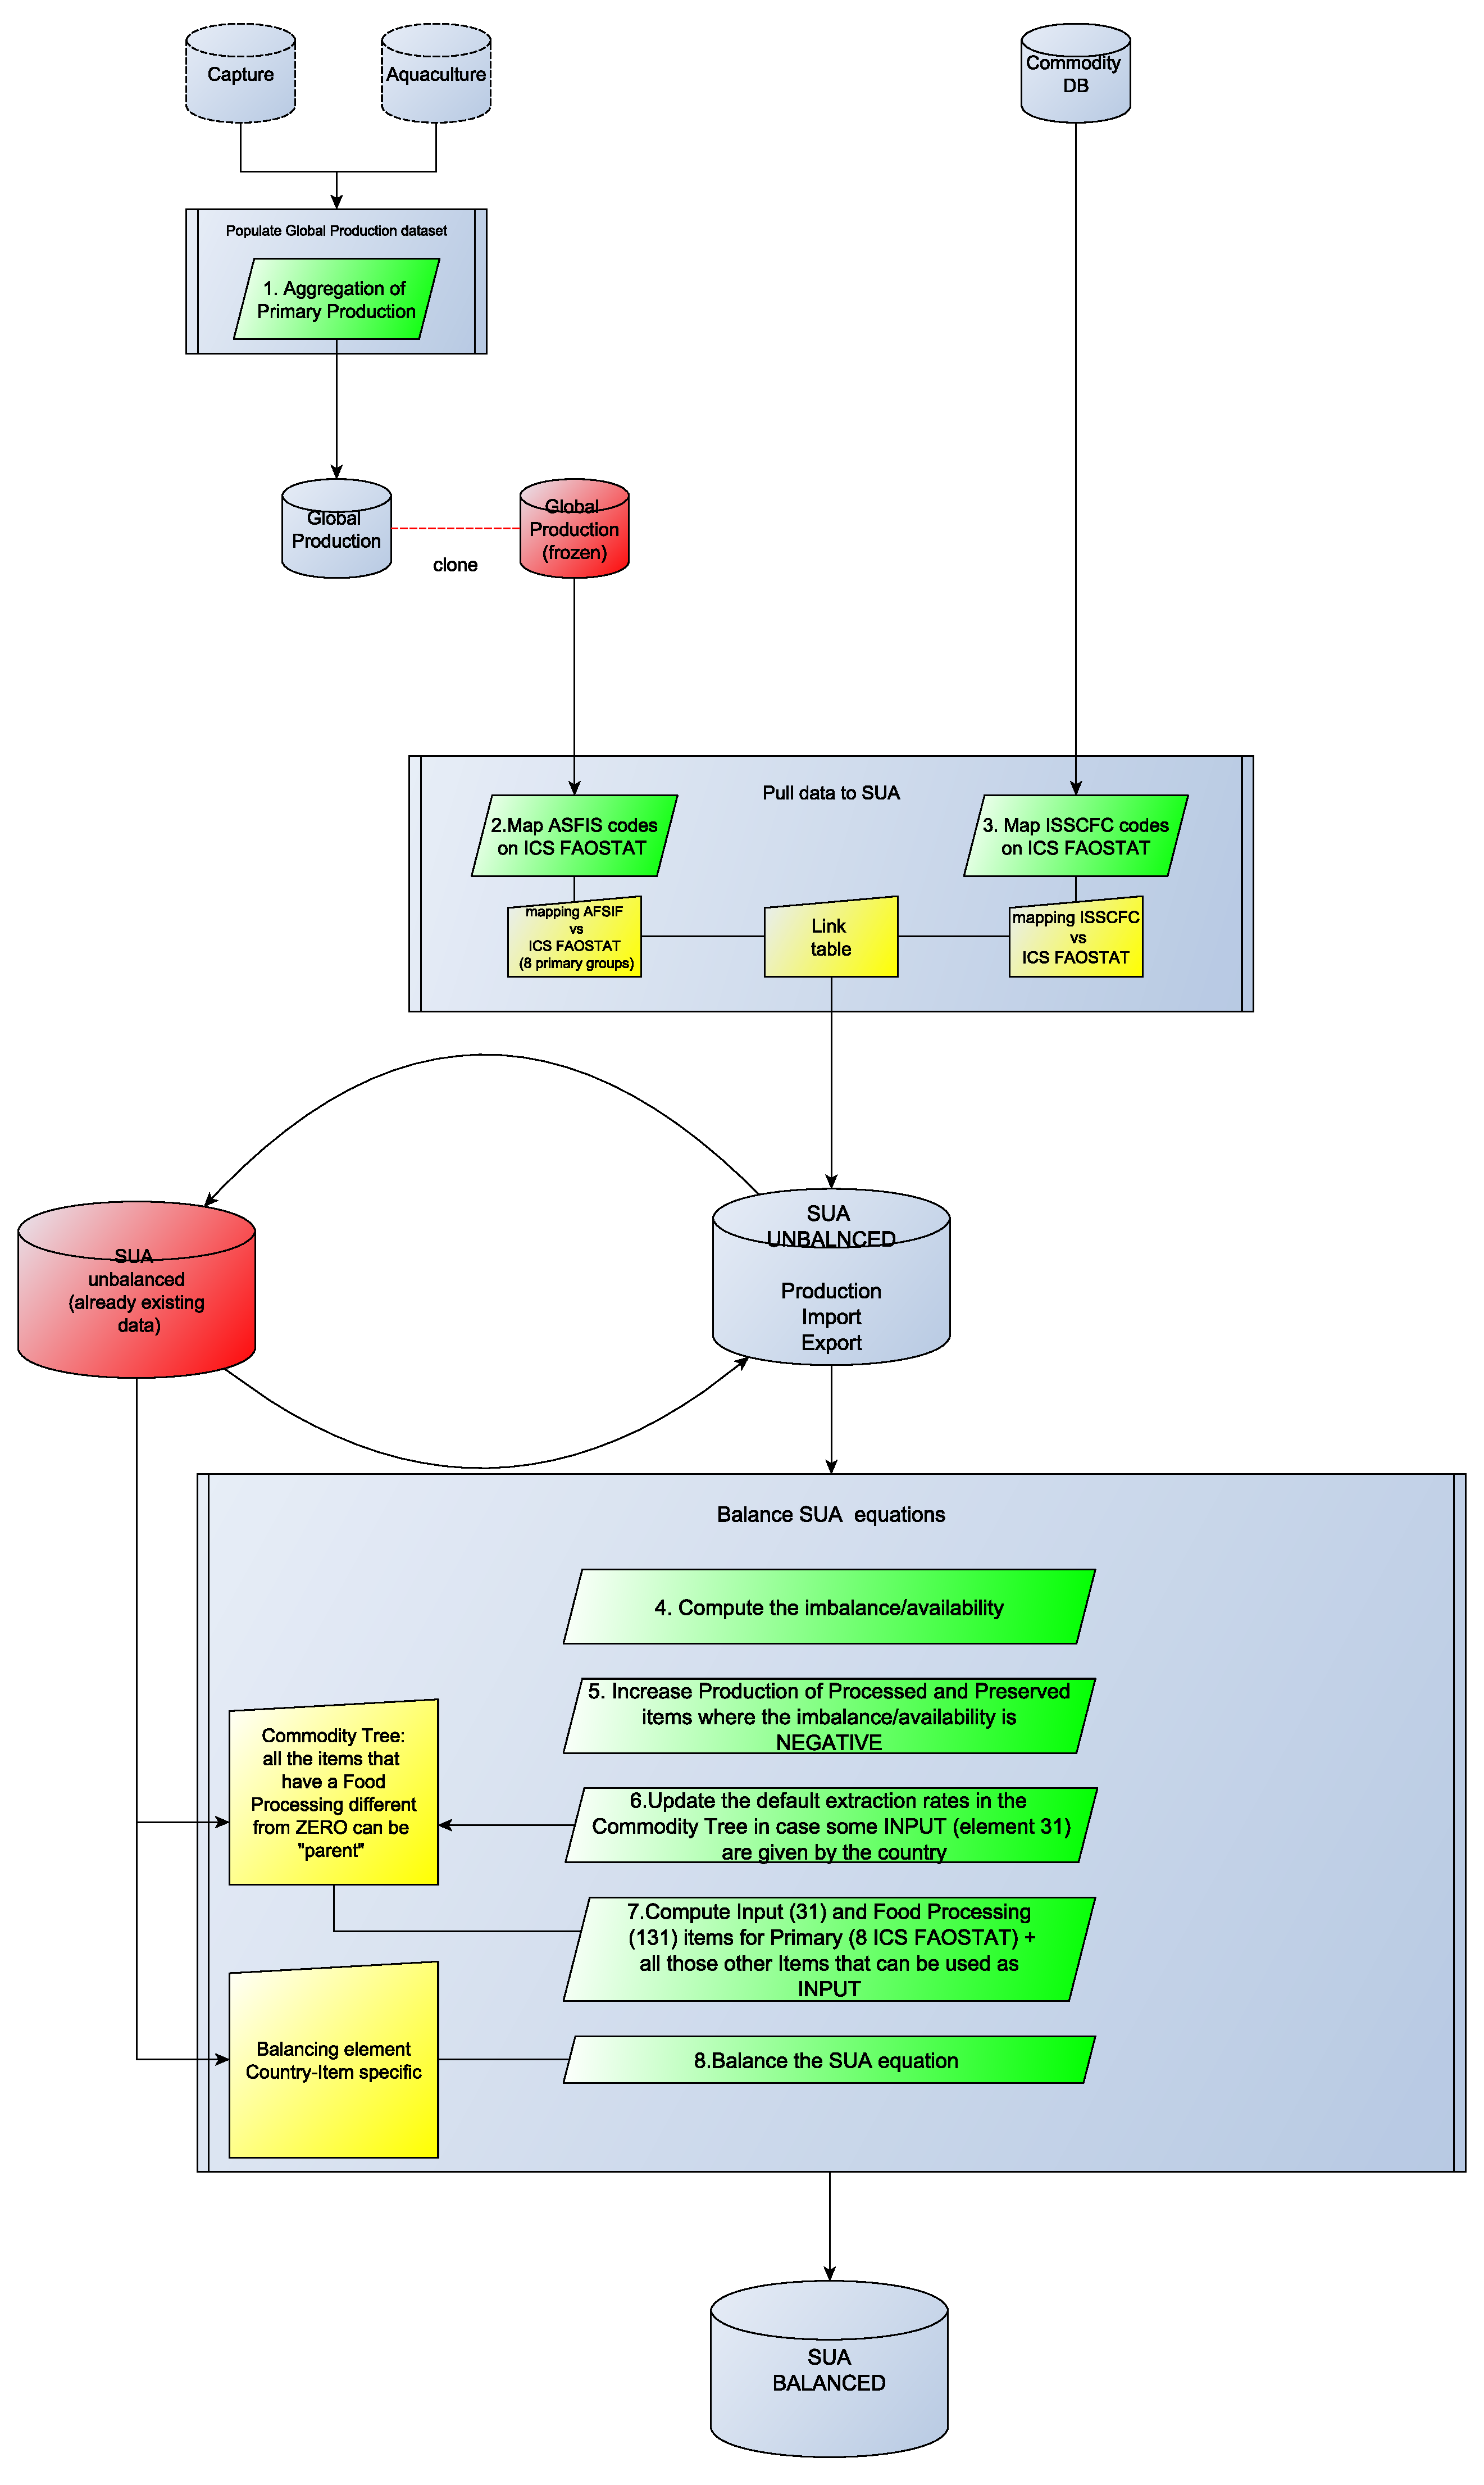
\includegraphics{flow-charts/pullDataToSUA/pullDataToSUA_globalProdFROZEN.pdf}
\caption{Overall workflow}
\end{figure}




\section {FIAS datasets - migration to the SWS}

\subsection{Global Production}
Primary Production data for Fishery products may come from both Capture and Aquaculture. Capture and Aquaculture data are collected and stored in two different SWS datasets. Data is collected via FIAS questionnaire and it is consolidated and fully validated thanks an intense activity of research on the web and on official publications.

The Global Production data set is considered reliable enough to be autonomously disseminated. It basically represents the starting point to compute FBS and, together with the Commodity DB (see Section 2.2.) it is used to compile the primary availability, which is the amount of primary product allocated as input for any productive processes which lead to the production of processed and preserved items.

Both capture and aquaculture data are collected according to the ASFIS list of Species for Fishery Statistics Purposes. 

\paragraph{Primary production - ASFIS classification}

For each species, the following descriptors are provided: 

\begin{itemize}
\item \textbf{3-alpha code}: classification issues only for species of commercial significance. Its codes have a predefined structure: three alphabetic characters that represent a very short abreviation of the name of the species\footnotes{ It is used in tables, questionnaires and publications in which the lack of space may impede the use of adequate descriptors in all the languages}. FAO is the depository agency for the 3-alpha codes: all requests for information and for the allocation of a 3-alpha code to new species should be addressed to FAO. 


\item \textbf{Taxonomic code}: hierachical classification consisting of five levels of aggregation (Main groupings, Orders, Families, Genera and Species). It contains also several attributes for each code: scientific name, author(s), family \dots
\end{itemize}

All species in the ASFIS list are classified by \textbf{ISSCAAP group}, with the exception of marine birds and snakes. The International Standard Statistical Classification for Aquatic Animals and Plants (ISSCAAP) classifies aquatic commercial species into 50 groups and nine divisions on the basis of their taxonomic, ecological and economic characteristics. The ISSCAAP groups are used to aggregate ASFIS items into macro-categories and to finally map ASFIS codes onto ICS FAOSTAT groups.


\paragraph{Aggregation of Capture and Aquaculture into the Global Production dataset - }
Capture and Aquaculture datasets are consistent in terms of classifications, but are not completely consistent in terms of dataset dimensions. Aquaculture has one more data dimension: Production Source (brackishwater, freshwater, marine)\footnote{Note that the term dimension is used the identify the dataset columns whose combintion univocally identifies a data-point.}.
Once both Capture and Aquaculture data have been validated, the two datasets are aggregated to populate the Global Production SWS dataset. 
This procedure includes the following steps:
\begin{itemize}
\item Aggregate the Aquaculture data by ''Production source'' in order to remove the dimension ''Production Source'' and make the both Aquaculture and Capture dataset compliant in terms of dataset-dimentions.
\item Furtherly aggregate by species the amount of production  coming from Capture with the amount coming from Aquaculture in order to have, at country level, one unique figure referring to the primary production for each species by fishing Area, on a yearly basis.

\end{itemize}
The routine to properly aggregate Capture and Aquaculture dataset has been already uploaded in the SWS (as a R plugin). It has been developed by FIAS teams\footnote{Thomas Berger is the focal point - plugin in Prod env: \textit{Global Production}.}.

As shown in the \textit{Overall workflow} flowchart, \textit{Global Production} dataset (obtained as result of the this aggregation) is frozen and cloned. The cloned \textit{Global Production} dataset is a separate envirnoment and it is a perfect copy of the \textit{Global Production} dataset currently released. This step ensures to FIAS team to keep working on the Global Production dataset without interfeering with the activities related to the FBS compilation. This latter version of the \textit{Glabal Production} dataset which is fully validated, released and frozen, is used as input to produce the FBS. This dataset has the structure reported in Table 1.

\subsection {The Commodities DB}
The socalled  Commodities database contains mainly trade data, anyway it also contains production of processed and preserved commodities \footnote{For a comprehensive discussion about the Commodity DB and its production component, make reference to the document \textit{Production of processed and preserved items in the Commodity DB}}.

Items are classified according to the International Standard Statistical Classification of Fisheries Commodities (ISSCFC). It covers products derived from fish, crustaceans, molluscs and other aquatic animals, plants and residues. This classification is based on the structure of the United Nations Standard International Trade Classification (SITC), with additional codes to include links to ISSCAAP and breakdown by additional species and product forms. It includes links to the Harmonized System classification (HS) and to the Central Product Classification (CPC). In the ISSCFC, fisheries and aquaculture commodities are classified according to the species and to the degree of processing undergone.

As aready mentioned, this dataset (together with the Primary Production) is used as input to the FBS compilation. While the trade components (Import and Export) are cosidered relieable enough and cannot be modified by the Standardization procedure\footnote{Procedure to convert all the processed }, the Production component of the Commodity Database can be readjusted.

\begin{landscape}
\begin{table}[t]
\caption{Global Production - dataset structure}
\centering
\begin{tabular}{c|c|c|c|c|c|c|c}
\toprule
geographicAreaM49 & fisheriesAsfis & fisheriesCatchArea & measuredElement & timePointYears & Value & flagObservationStatus & flagMethod\\
\midrule

itme1 & 36.101954 & 45 & 0.825500 & 0.220198 & 0.293448 & x & y \\
item2 & 51.828572 & 45 & 0.224900 & 0.499718 & 0.690064& x & y \\

\bottomrule
\end{tabular}
\label{tab:xxx}
\end{table}


\end{landscape}



\subsection{SUA unbalanced}
Once \textit{Global production} and \textit{Commodity DB} data has been reconciled, production and trade flows, properly associated to \textit{ICS FAOSTAT} groups, populate the \textit{SUA unbalanced} table.

The R routine to update the already existing SUA tables is generally referred as the \textit{Pull data to SUA}\footnote{Please note that the \textit{Pull Data to SUA} operation is currently the first part of the routine developed to compile FBS}.

Given that the SUA had been already compiled in the past, the socalled SUA unbalanced table, actually contain the SUA equations that had been already balanced at least up to the last release of the FBS. In other words, the first time the SUA unbalanced table is popultaed, existing SUA tables (already balanced) should be included in the SWS dataset. 

Each time the \textit{Pull data to SUA} routine is run, the updated figures are highlighted (red triangle in the corner of the cell) and the user can easily visualize which figures had changed.


The migration of current SUAs tables into the SWS request the mapping of the current element codes onto the SWS element list. Table 2. contains the first draft proposal to convert current FIAS SUAs into the SWS SUA unbalanced table.


\begin{table}[t]
\caption{Proposal: mapping of the current FIAS element codes onto the SWS element codes.}
\centering
\begin{tabular}{c|c|c|c}
\toprule
FIAS code  & label & proposed code & proposed label                    \\
\midrule

51   &	Production     & 5510 & Production                             \\
61   &	Imports - Qty  & 5610 & Import Quantity [t]                    \\
62   &	Imports - Val  &      &                                        \\

91   &	Exports - Qty  & 5910 & Export Quantity [t]                    \\
92   &	Exports - Val  &      &                                        \\
                  
101   &	Feed           & 5520 & Feed [t]                               \\
111   &	Breed/Bait     &      &                                        \\
                  
121   &	Waste          &    5016 & Waste [t]                           \\
131   &	Processing     &    5023 & Processed [t]                       \\
141   &	Food           &    5141 & Food [t]                            \\
151   &	Other Util     &    5166 & Residual other uses [t]             \\
                  
31   &	Input          &                     &                         \\
41   &	Extr Rate      &                     &                         \\ 

71   &	Stock Variation   &   5071 & Stock Variation [t]               \\
77   &	Cumulative Stocks &        &                                   \\

261   &	Food: Total Calories Eqv  &     &                  \\ 
264   &	Calories/Caput/Day        & 664 & Food supply (/capita/day)[kcal] \\             
271   &	Food: Total Proteins Eqv  &     &                  \\    
274   &	Proteins/Caput/Day        &     &                  \\      
281   &	Food: Total Fats Eqv      &     &                  \\    
284   &	Fats/Caput/Day            &     &                  \\    

\bottomrule
\end{tabular}
\label{tab:xxx}
\end{table} 





\section {The methodology}


The overall workflow to compile Food Balance Sheets fosees several R plugins that populate different SWS datasets or a single plugin that dave in different datasets intermediate output (\textit{sua unbalanced}, \textit{sua balanced}, \textit{fbs standardized} and any other intermediate output that might be useful for validation purposes). This choice should facilitate the data-validation procedure. The FBS officer can check the output of each sub-module and eventually manually interveene if ad hoc adjustements are required. 


The following sessions are addressed to provide details about the R modules under develpment to trasform the input data (\textit{Primary Production} dataset and the \textit{Commodity DB} into the \textit{Fishery Food Balance Sheets}).



\subsection{Populate the SUA unbalanced table: the ICS FAOSTAT classification}
To build the Supply-Utilization Account dataset, it is necessary to reconcile the information coming from the Primary Production and from the Commodity Database. Items, in these two datasets, are classified according to different classifications, ASFIS and ISSCFC respectively. This means that \textit{primary production}  and \textit{trade} data are characterized by a different level of detail in terms of species classification.

On the other hand, SUA equations are associated to ICS FAOSTAT groups. This means that fish and fish products contained in each ICS item do not represent individual species or commodities, but the aggregation of different species and products. About 2 000 species produced and 1 000 items traded are conveyed into 8 main groups of similar biological characteristic \footnote{Currently the SUAs/FBS for aquatic plants are not calculated (with the exception of three countries in FAOSTAT) due to the lack of separate data for edible/non-edible trade until recently. Due to the improvement of the HS classification and the introduction of specific codes distinguishing edible from non-edible aquatic plants/seaweed, this could change in the near future.}, reflecting the ISSCAAP classification,  with further breakdowns associated to processed and preserved commodities.

The main eight groups of species forming SUAs and FBS for fish and fishery products are: 
\begin{itemize}
\item Freshwater and Diadromous fish;
\item Demersal fish;
\item Pelagic fish;
\item Marine fish other; 
\item Crustaceans; 
\item Molluscs, excluding cephalopods; 
\item Cephalopods; 
\item Other aquatic animals.
\end{itemize}

These eight ICS groups are looked as primary items: there is a one to one relationship between between the primary ICS groups and the final  FBS groups. Table 3. shows this one to one correspondence.

\begin{table}[t]
\caption{ICS - FBS mapping}
\centering
\begin{tabular}{c|c|c}
\toprule
geographicAreaM49 & fisheriesAsfis & fisheriesCatchArea \\
\midrule

       010 &  1501    & Freshwater and Diadromous fish; \\
       020 &  1514    & Demersal fish;                  \\ 
       030 &  1527    & Pelagic fish;                   \\
       040 &  1540    & Marine fish other;              \\
       050 &  1553    & Crustaceans;                    \\
       060 &  1562    & Molluscs, excluding cephalopods \\  
       070 &  1570    & Cephalopods;                    \\
       090 &  1594    & Other aquatic animals.          \\

\bottomrule
\end{tabular}
\label{tab:xxx}
\end{table}


\begin{figure}
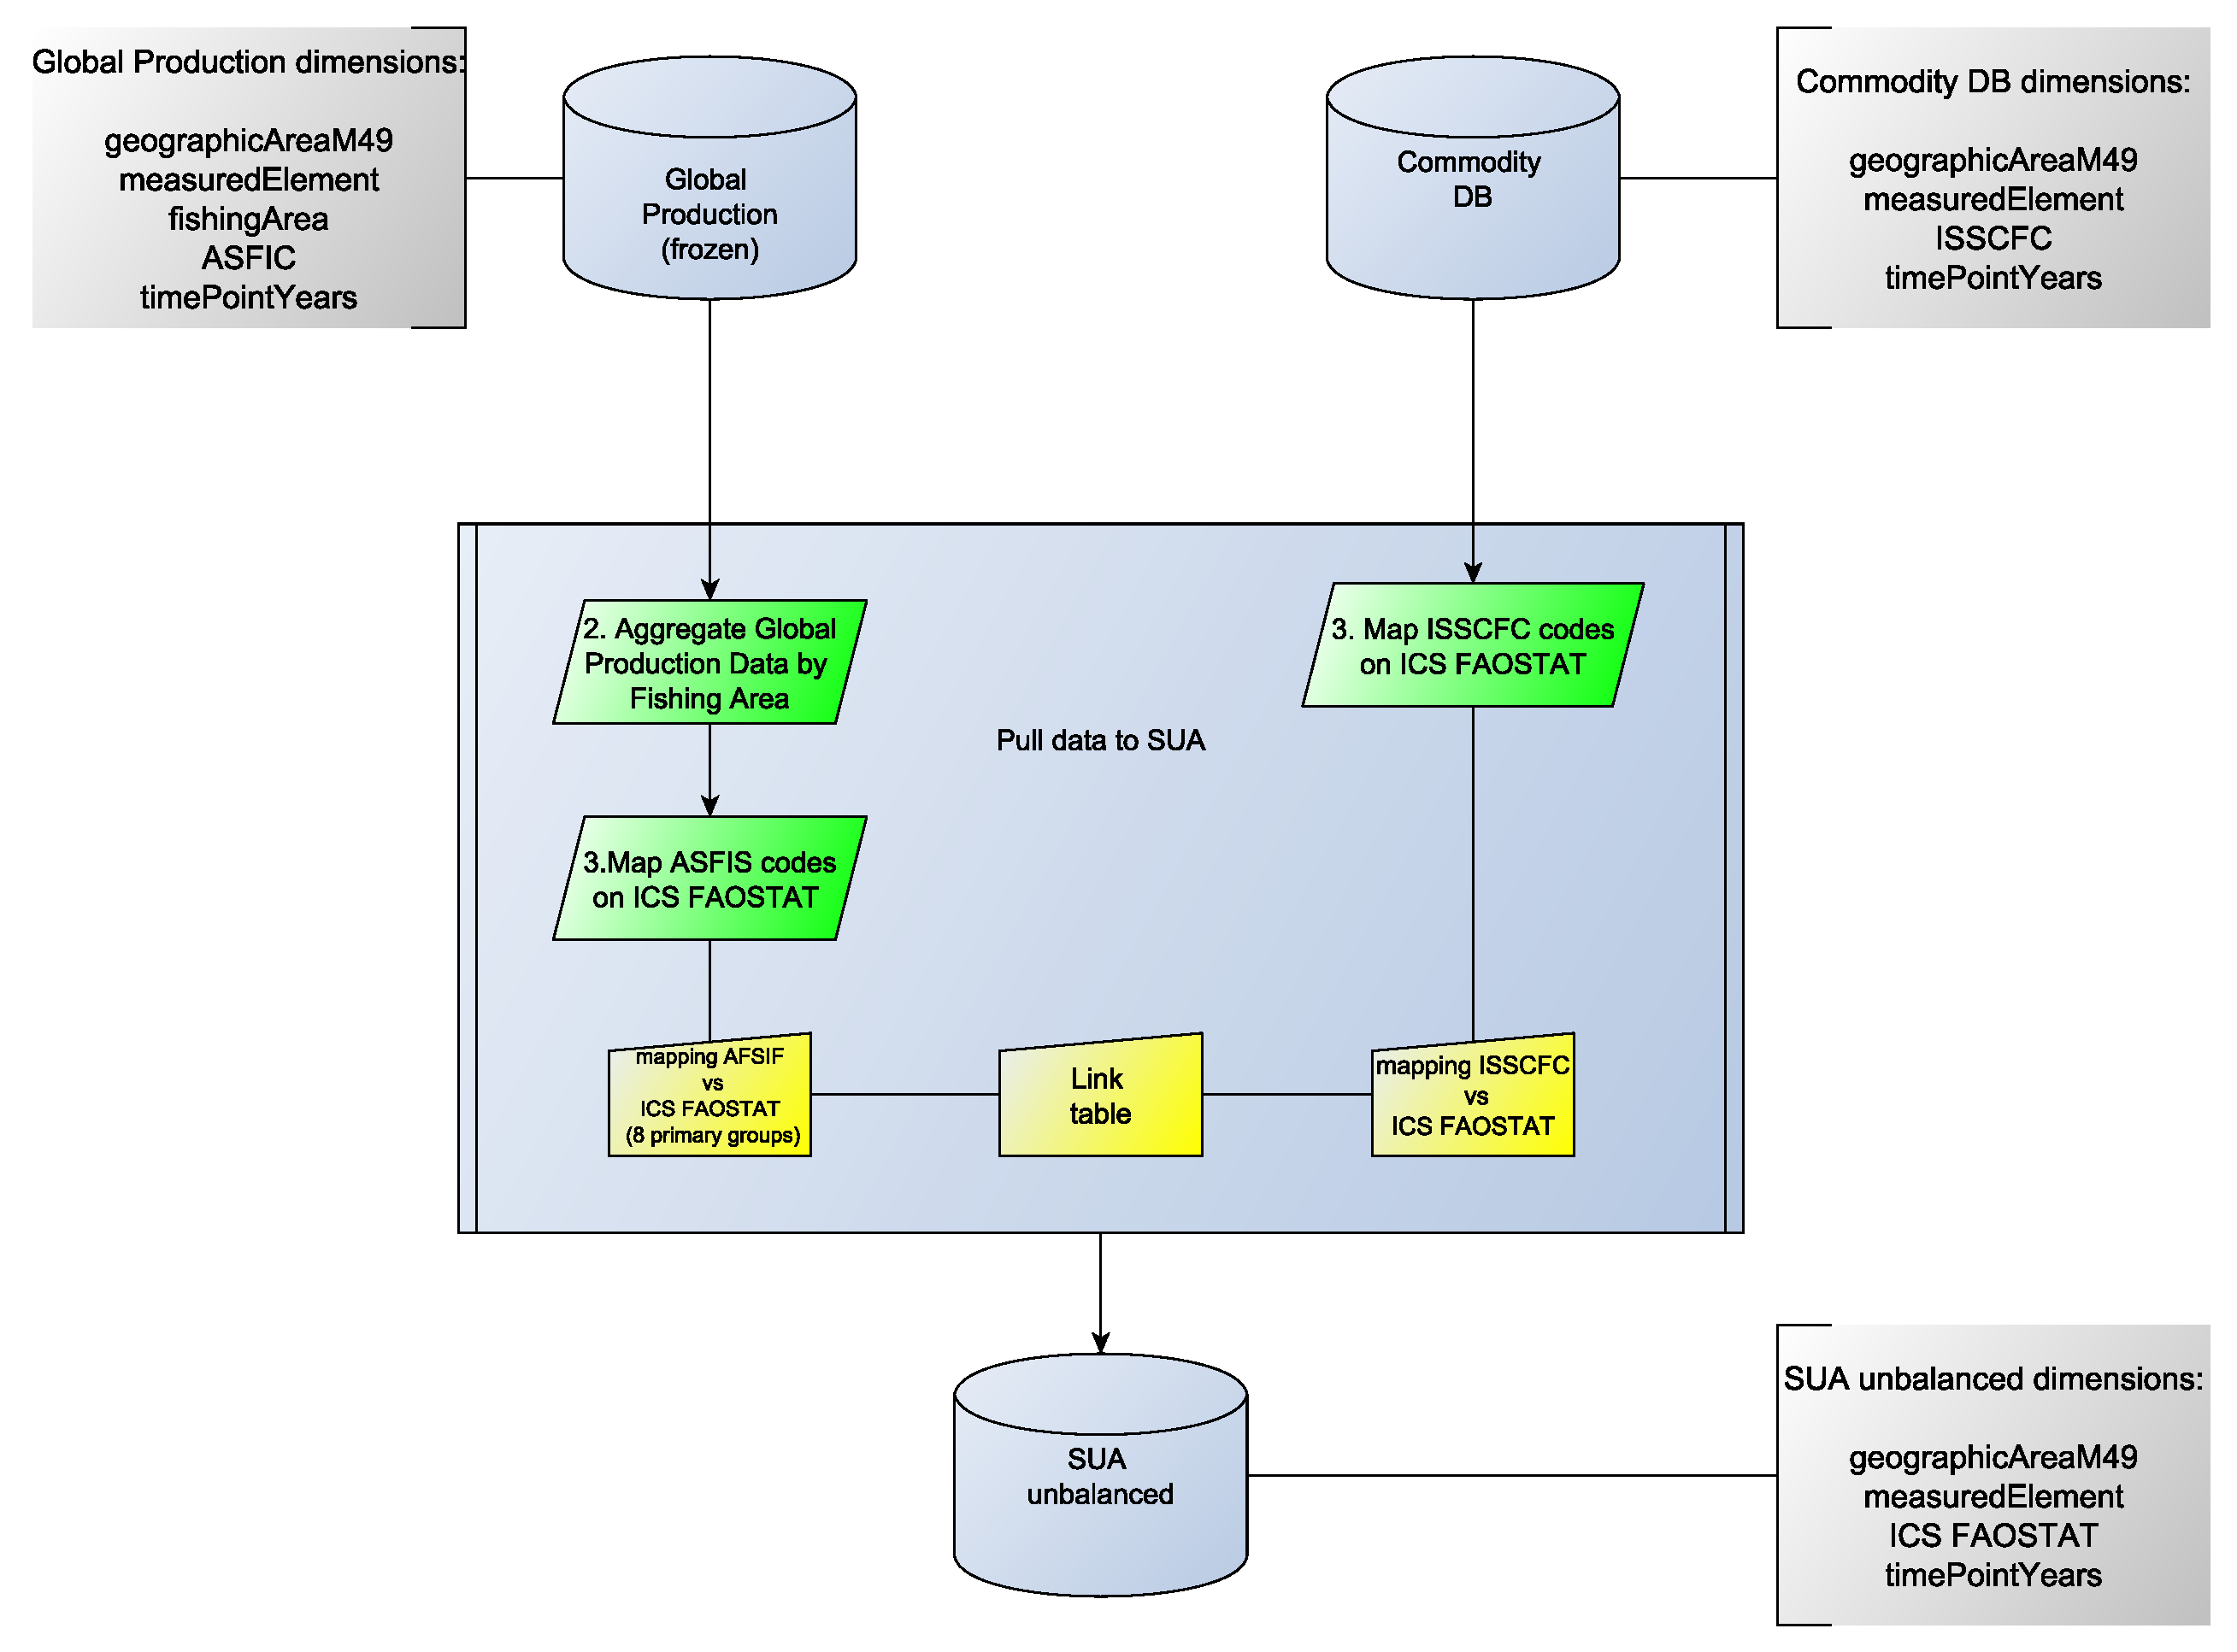
\includegraphics{flow-charts/pullDataToSUA/focusOnCompileSUA_Unbalanced.pdf}
\caption{Pull data to SUA: reconcile Global Production Data with the Commodity DB.}
\end{figure}


Figure 2. summarizes the overall workflow and reports the auxiliary-files (generally stored as data-tables in the SWS) to perform the mapping. The proper mapping tables, had been built to aggregate Primary Items (ASFIS) into the 8 primary ICS groups and the \textit{Commodity DB} items (ISSCFC) into the proper ICS group.

\paragraph{Example: ASFIS - ICS mapping}

Table 4. contains an example refferring to the composition in terms of ASFIS codes of the ISSCAAP group \textit{Carps, barbels and other cyprinids (11)} for Russia - 2014. The table also shows how all the ASFIS items associated to the eleventh ISSCAAP group are aggregated into the ICS group \textit{Freshwater & diadromous fish, fresh}(1501):

\begin{landscape}
\begin{table}[t]
\caption{ICS - FBS mapping}
\centering
\begin{tabular}{c|c|c|c|c|c|c}
\toprule
geographicAreaM49 & fisheriesAsfis & measuredElement & timePointYears & Value & isscaap & ics \\
\midrule
643   &  ABK    & 5510 & 2014 &   7193   & 11 &  1501 \\
643   &  ASU    & 5510 & 2014 &   424    & 11 &  1501 \\ 
643   &  BKC    & 5510 & 2014 &   0      & 11 &  1501 \\
643   &  CGO    & 5510 & 2014 &   0      & 11 &  1501 \\
643   &  FBM    & 5510 & 2014 &   20673  & 11 &  1501 \\
643   &  FBR    & 5510 & 2014 &   3908   & 11 &  1501 \\  
643   &  FCC    & 5510 & 2014 &   0      & 11 &  1501 \\
643   &  FCG    & 5510 & 2014 &   19468  & 11 &  1501 \\
643   &  FCP    & 5510 & 2014 &   63249  & 11 &  1501 \\
643   &  FCY    & 5510 & 2014 &   30498  & 11 &  1501 \\ 
643   &  FID    & 5510 & 2014 &   5930   & 11 &  1501 \\
643   &  FRO    & 5510 & 2014 &   758    & 11 &  1501 \\
643   &  FRX    & 5510 & 2014 &   17603  & 11 &  1501 \\
643   &  FSC    & 5510 & 2014 &   2751   & 11 &  1501 \\  
643   &  FTE    & 5510 & 2014 &   1134   & 11 &  1501 \\
643   &  SRE    & 5510 & 2014 &   8872   & 11 &  1501 \\
643   &  SVC    & 5510 & 2014 &   23315  & 11 &  1501 \\

\bottomrule
\end{tabular}
\label{tab:xxx}
\end{table}
\end{landscape} 



\subsubsection{The Link table}

Sometimes the default mapping tables do not provide the proper aggregations of ASFIS or ISSCFC codes into ICS groups. This means that some already agreggated flows have to be migrated from the default ICS group to an ad hoc one. These exceptions are counry- year specific and a data-table \footnote{domain: fisheries, datatable: \textit{link_mapping}} has been created to host this information in a such a way as to be easily digest by the R script on one hand, and easily read and updated by any FIAS user on the other.


The \textit{deviation} of any ICS aggregated flow to another, is typically based on a one to one relationship. Anyway, sometimes it is necessary to split the aggregated ICS flow into two or more alternative ICS groups. One to many relationships need an additonal information: the percentage to split one ICS flow into many\footnote{Embedded in the R routine there are also several checks to ensure that the sum of these percentage by \textit{from_code} always sum to one. }.  This additional information is contained in the \textbf{Link table} whose extraction of few lines is here reported:


\begin{Schunk}
\begin{Soutput}
   geographic_area_m49 flow start_year end_year from_code percentage to_code
1:                   8  EXP       1991     LAST      1541          1    1515
2:                   8  EXP       1990     LAST      1545          1    1532
3:                   8  EXP       1976     1995      1554          1    1562
4:                   8  PRD       1991     LAST      1541          1    1515
5:                   8  PRD       1990     LAST      1545          1    1532
\end{Soutput}
\end{Schunk}



The \textfb{Link} table is represented in the workflow (Figure 1.) as an \textit{ad hoc adjustment file} which can be manually compiled and updated: the user can manually populate the ''ad hoc adjustment file'' and re-run the R-routine. 


\subsection{Adjust the Production component of processed and preserved items}

As already mensioned, while primary production data is considered fully validated and cannot be re-adjusted, the production componenet associate to processed and preserved ICS groups (frozen, cured, canned ,meals, offals..) is systematically increased if the resulting net trade is negative .

Let's take into account a concreete example: once the \textit{SUA unbalanced} table has been populated, for each ICS group the following SUA components might be available:


\begin{itemize}

\item 51 - Production      -     5510 - Production                         
\item 61 - Imports - Qty   -     5610 - Import Quantity [t]                
\item 91 - Exports - Qty   -     5910 - Export Quantity [t]                
\item 101 - Feed           -    5520  - Feed [t]                            
\item 111 - Breed/Bait     -     
\item 121 -	Waste          -    5016  - Waste [t]                          
\item 141 -	Food           -    5141  - Food [t]                           
\item 71  -	Stock Variation -   5071  - Stock Variation [t]               
\end{itemize}

Note that only \textit{production} (5510) and \textit{trade} (5610-5910) come from the \textir{Global Production - Frozen} and the \textit{Commodity DB} respectively. The presence of any other component may come only from:

\begin{itemize}
\item FIAS questionnaire (if available);
\item expert evaluation;
\item manual entry of the figures stored in the \textit{disposition} dataset;
\item publications, field missions.
\end{itemize}

Considering an example where only production, import and export are available\footnote{Likely inutial configuration for many items.}, the availability is obtained as:

$$
Production+Import-Export= availability
$$

If the just computed availability is negative, only for non primary items, the \textit{production component} is increased in order to balance the SUA equation.

$$
Production'=Production-availability
$$

This operation ensures that no negative availabilities enters the next steps of the process.




If the availability of a primary ICS gruop\footnote{Freshwater and Diadromous fish; Demersal fish; Pelagic fish; Marine fish other; Crustaceans; Molluscs, excluding cephalopodsCephalopods; Other aquatic animals.} is negative, the production component cannot be authomatically increased. The FIAS officer will be warned about an unfeasible SUA equation.

Negative primary availability is the typical diagnostic tool to identify suspicious SUA equations that might request a manual adjustment.

\begin{figure}
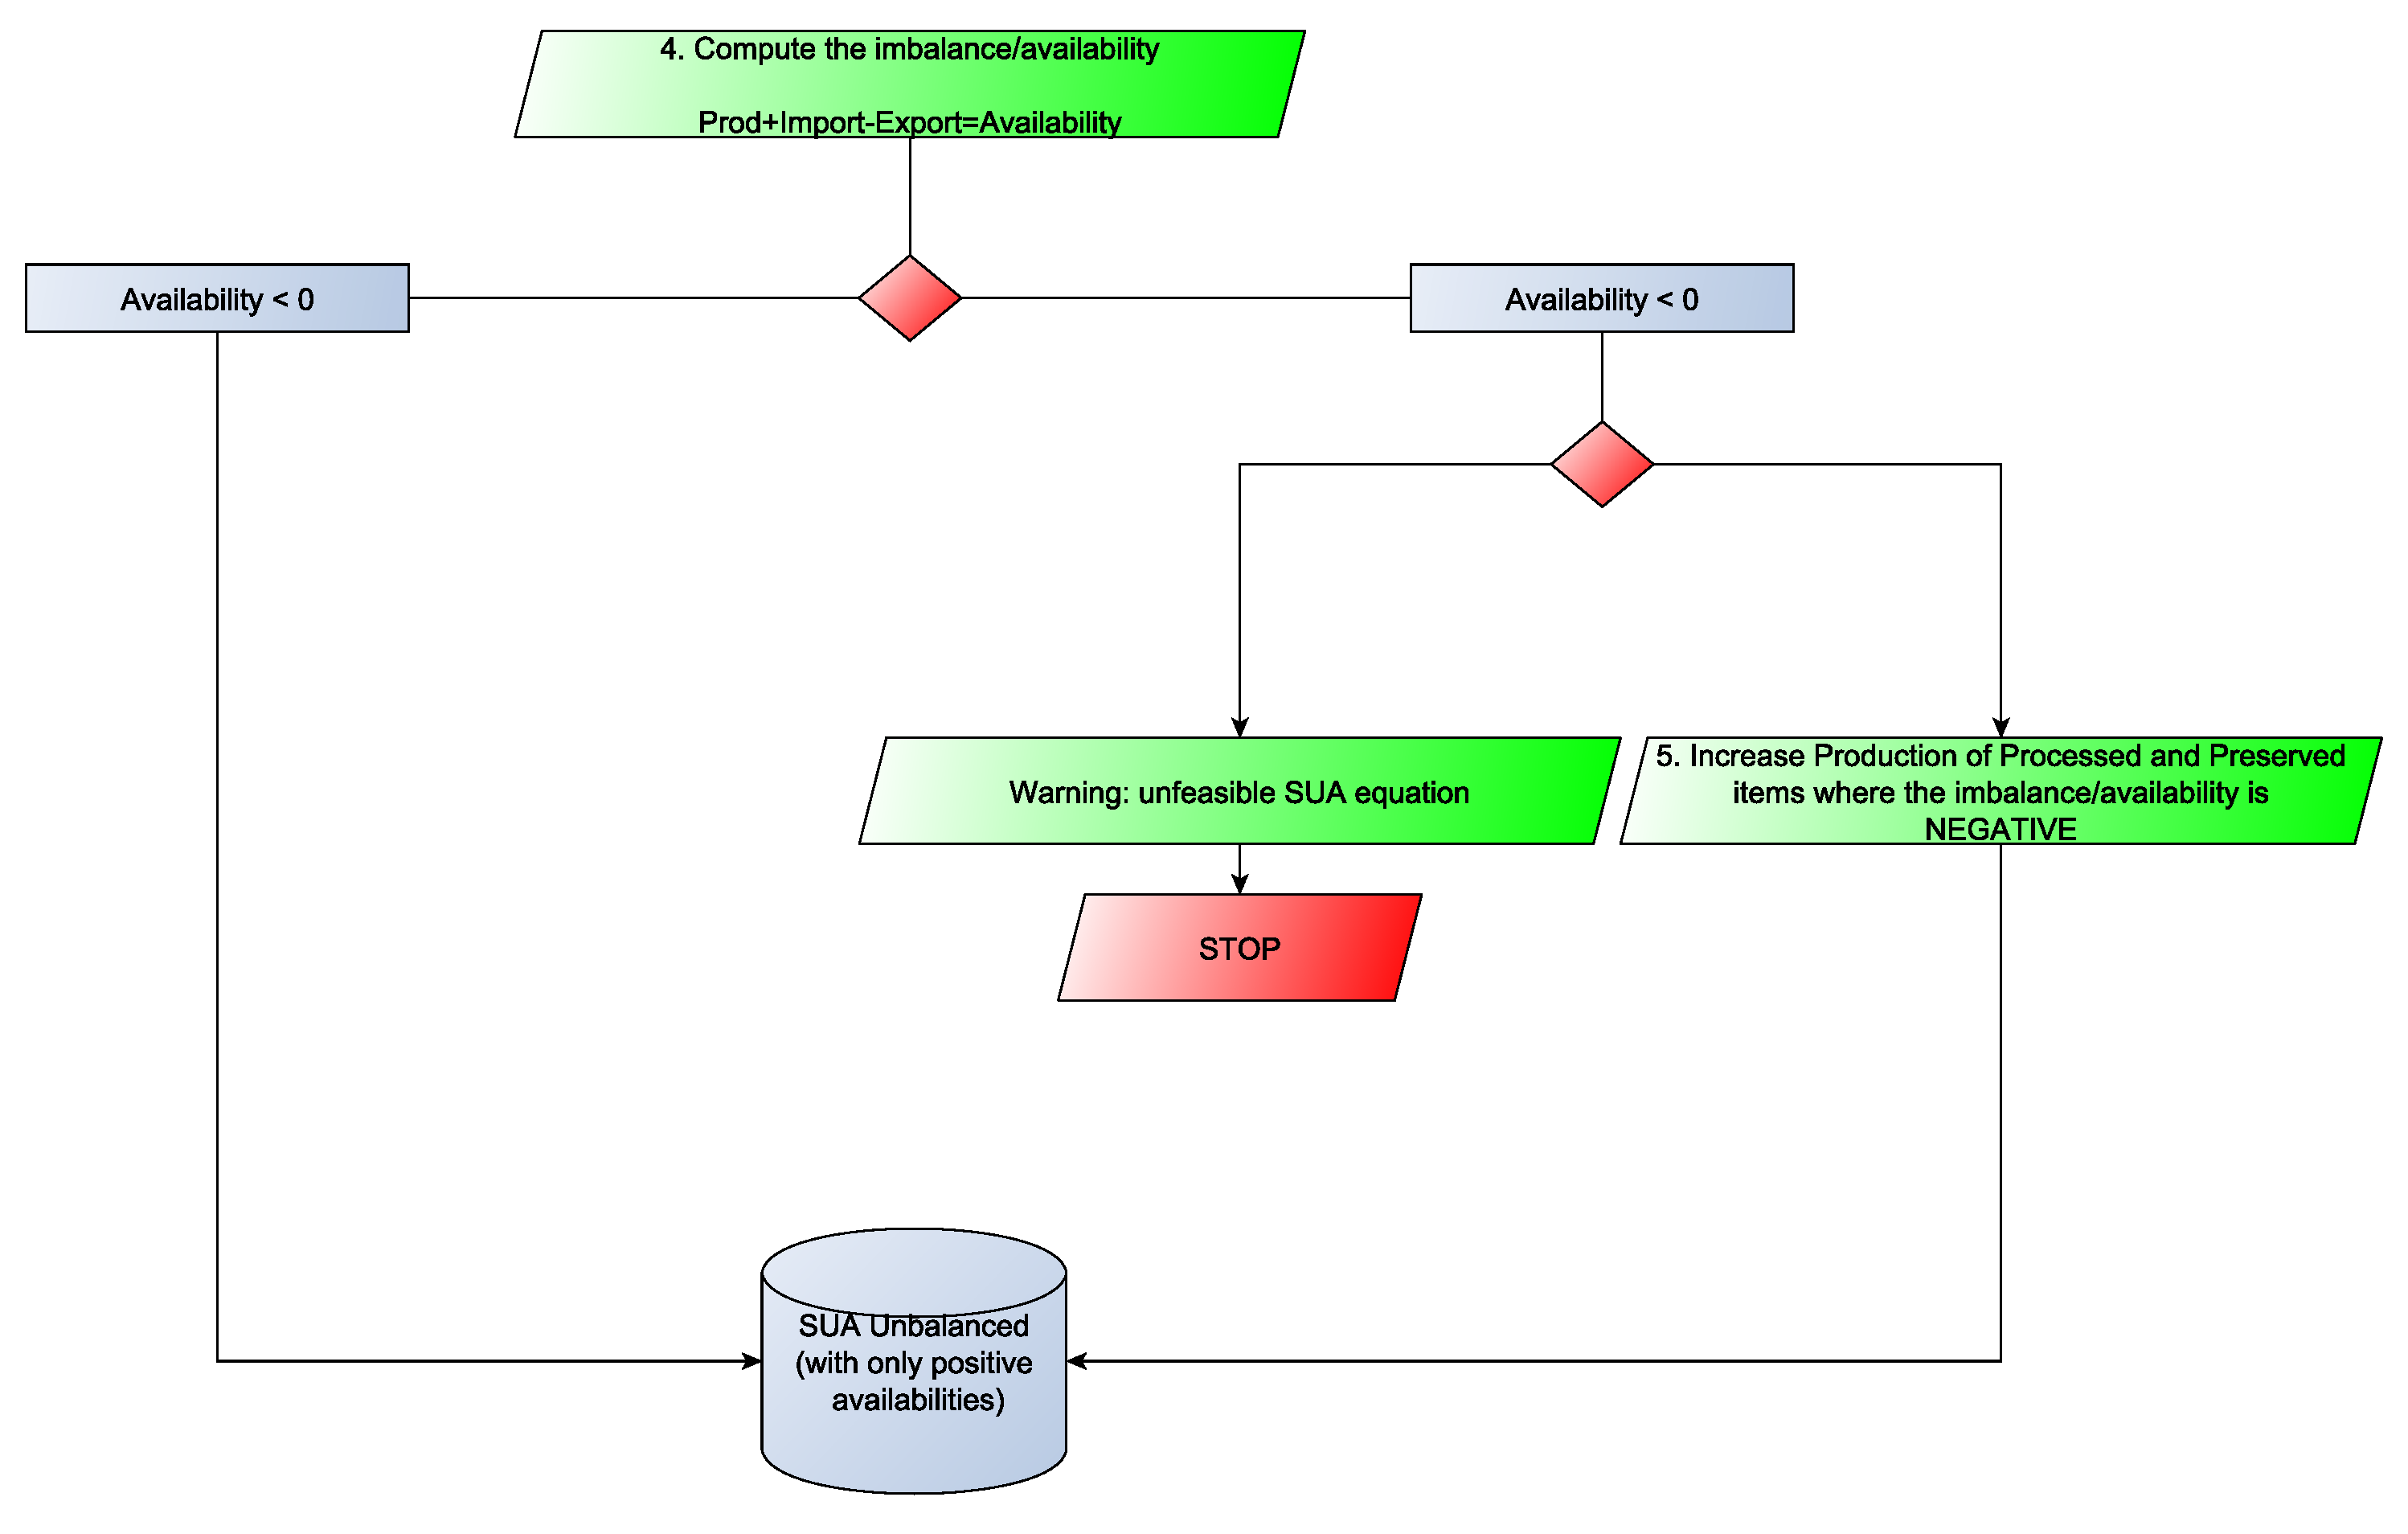
\includegraphics{flow-charts/balancing/balanceNegativeAvailability.pdf}
\caption{Adjust the Production component of processed and preserved items. Step 4. and step 5. are also highlighted in Figure 1. and can be contextualized in a broader flowchart.}
\end{figure}

Figure 3. summarise this procedure. 

\subsection{The food processing component}
Once the \texit{Production}  component has been increased (or filled) for all the processed commodities characterised by an initially negative imbalance, it is possible to compute the ''Food Processing'' component. This quantity represents the amount of each food item that is not consumed as it is, but it is allocated to one or more productive processes leading to one or more processed items. That's why to properly evaluate this component it is necessary to preliminary compile the ''production'' component for all the processed commodities. If one commodity is reported in the commodity tree as a final termination (cannot be used as input to produce any other processed items), the ''food processing'' component will obviously remain empty. In other words only those items that appear in the parent column of the commodity tree, are eventually characterized by a \textit{food processing} different than zero.

For those items that have several child-commodities the \textit{processing} component will be the sum of the partial contribution of each one of the processed items whose production has been obtained through a productive process that had, as input, the primary item taken in consideration. The partial contributions to the \textit{processing (element 131)} represent the amount of parent item necessary to produce each child separately. This amount is associated to each child item ( \textit{element 31, input}).


The country-year specific commodity tree has been build looking at the past SUA tables. The presence/absence of the \textit{Food processing} component -element 131- has been used to choose the connections to be  activated/cut.
Practically speacking, all those items characterized by an amount of  \textit{processing} different from zero in the past are eligible to play the role of \textit{parent} in the commodity-tree.

This conceptualization of the commodity tree and its representation in terms of dataset is an important improvement and provide the FBS Officer with a tool that automatically manages multi-level productiive processes. 




\subsubsection{The FIAS commodity tree}

Every primary product is the input for producing a broad variety of processed and preserved products. A modern food processing sector is characterized by a vast variety of different processed products.

The Standardization - the conversion and subsequent aggregation of processed products into their primary equivalents - aims to bring these products into a hierarchical order that reflects the various food processing chains in which primary products are converted into processed equivalents. The most straightforward way of depicting this hierarchy is in the form of commodity trees which contain a structured and clear set of relationships between commodities. 

Commodity trees are so-called because they ''stem'' from one primary product and then branch out into one or successive levels of processed products, each level is linked by extraction rates. Commodity trees are designed to be exhaustive, such that all possible uses of a particular commodity are covered. This means that they can be more or less complicated depending upon the number of derived products, the number of processing levels, and the creation of ''parallel-products'' during processing. 

As just mentioned, in the commodity-tree representation, each parent-child combination is characterized by an ''extraction rate''. Extraction rates reflect the amount of parent product contained in the next level of processed product; for instance, the extraction rate of \textit{Freshwater Fillets}  is about 0.4. This means that 1 tonne of \textit{Freshwater Diadromous Fresh } going through a country's fish-industry renders an average of 400 kg of fillests. The same industry also produces \textit{Freshwater Meals From Offals (1511)}, on average 170 kg per tonne of \textit{Freshwater Diadromous Fresh }. Extraction rates are exogenously assumed. In terms of a broader interpretation, the extraction rate is the component that summarises the overall level of technology associated to each productive process, so it is assumed to vary across countries and over time as consequence of improvements in the level of technology. Extraction rates should be periodically reviewed and updated to ensure they remain valid and reflect the real status of technology in the country. Extraction rates might also be computed as a ratio at the condition that the country provides the ammount of primary item involved in each productive process.

Each commodity tree is represented as Figure 4. where:
\begin{itemize}
\item	nodes represent commodities,
\item	edges represent production processes,
\item	joints indicate where a single production process creates more than one commodity. These commodities are referred as parallel-products.
\end{itemize}
When a single productive process leads to more than one processed item, the resulting two or more by-products are identified as parallel-products (or co-products). This means that from the same amount of parent-commodity it is possible to obtain several processed items. A common example of co-products are fillet and offals, the both deriving from the filleting process. A particular attention should be paid in standardize this kind of processed items: only one (out of two) processed items expressed in terms of its parent equivalent is sufficient to obtain the total amount of \textit{fish (fresh)} necessary to produce the both by-products. That is why  ''offals'' are generally assigned a weight equal to zero in the standardization process: this means that they are not standardized. A full list of commodity classified as co-product is available and embedded into the R routines in order to avoid double-counting.


\begin{figure}
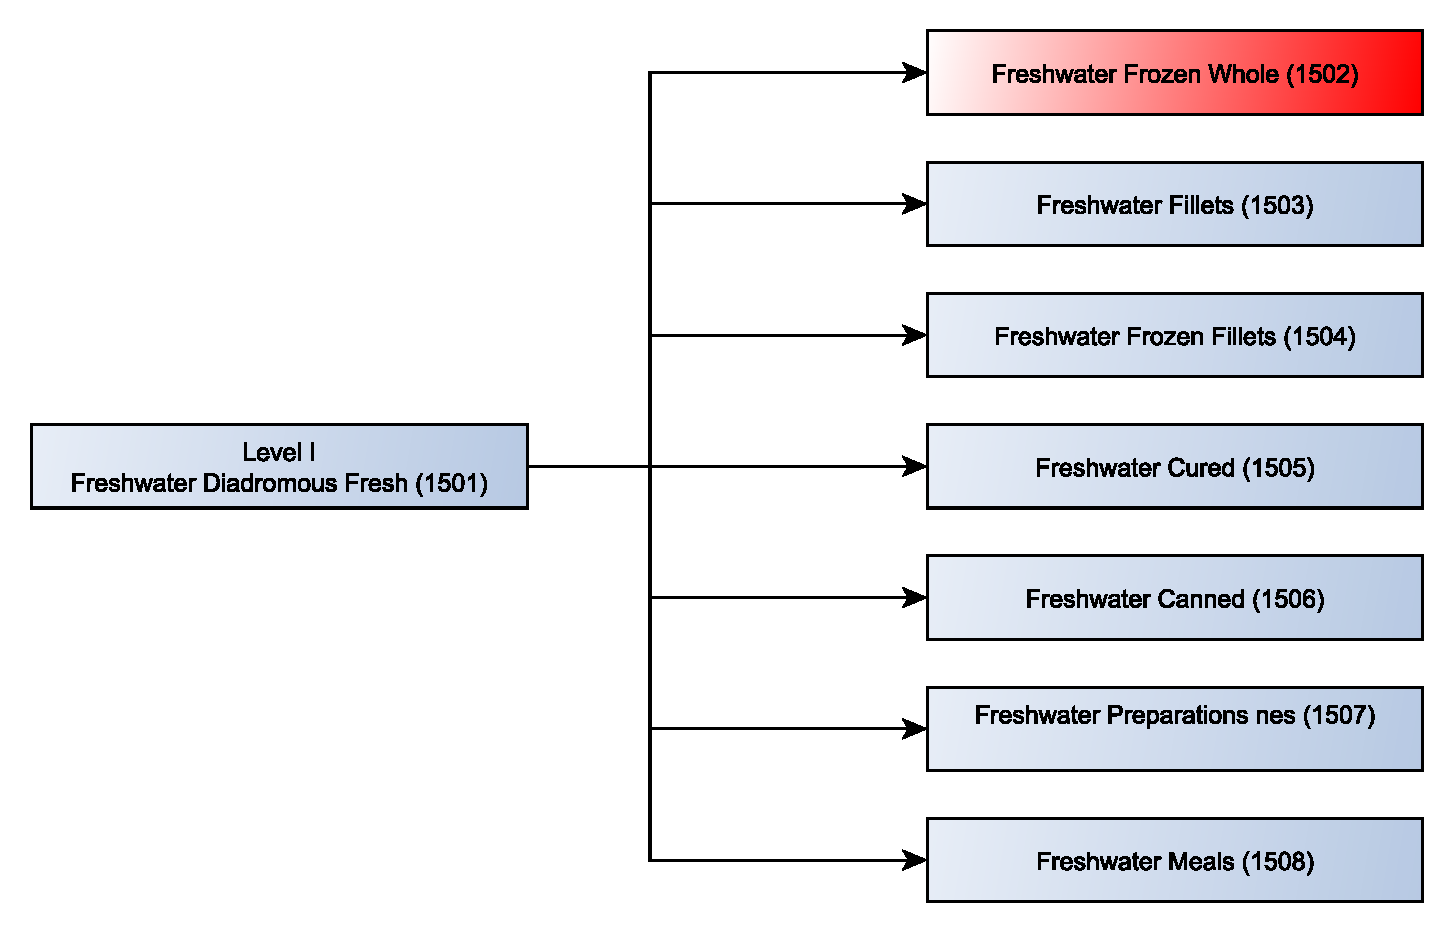
\includegraphics{flow-charts/tree/tree1501.pdf}
\caption{}
\end{figure}


\begin{figure}
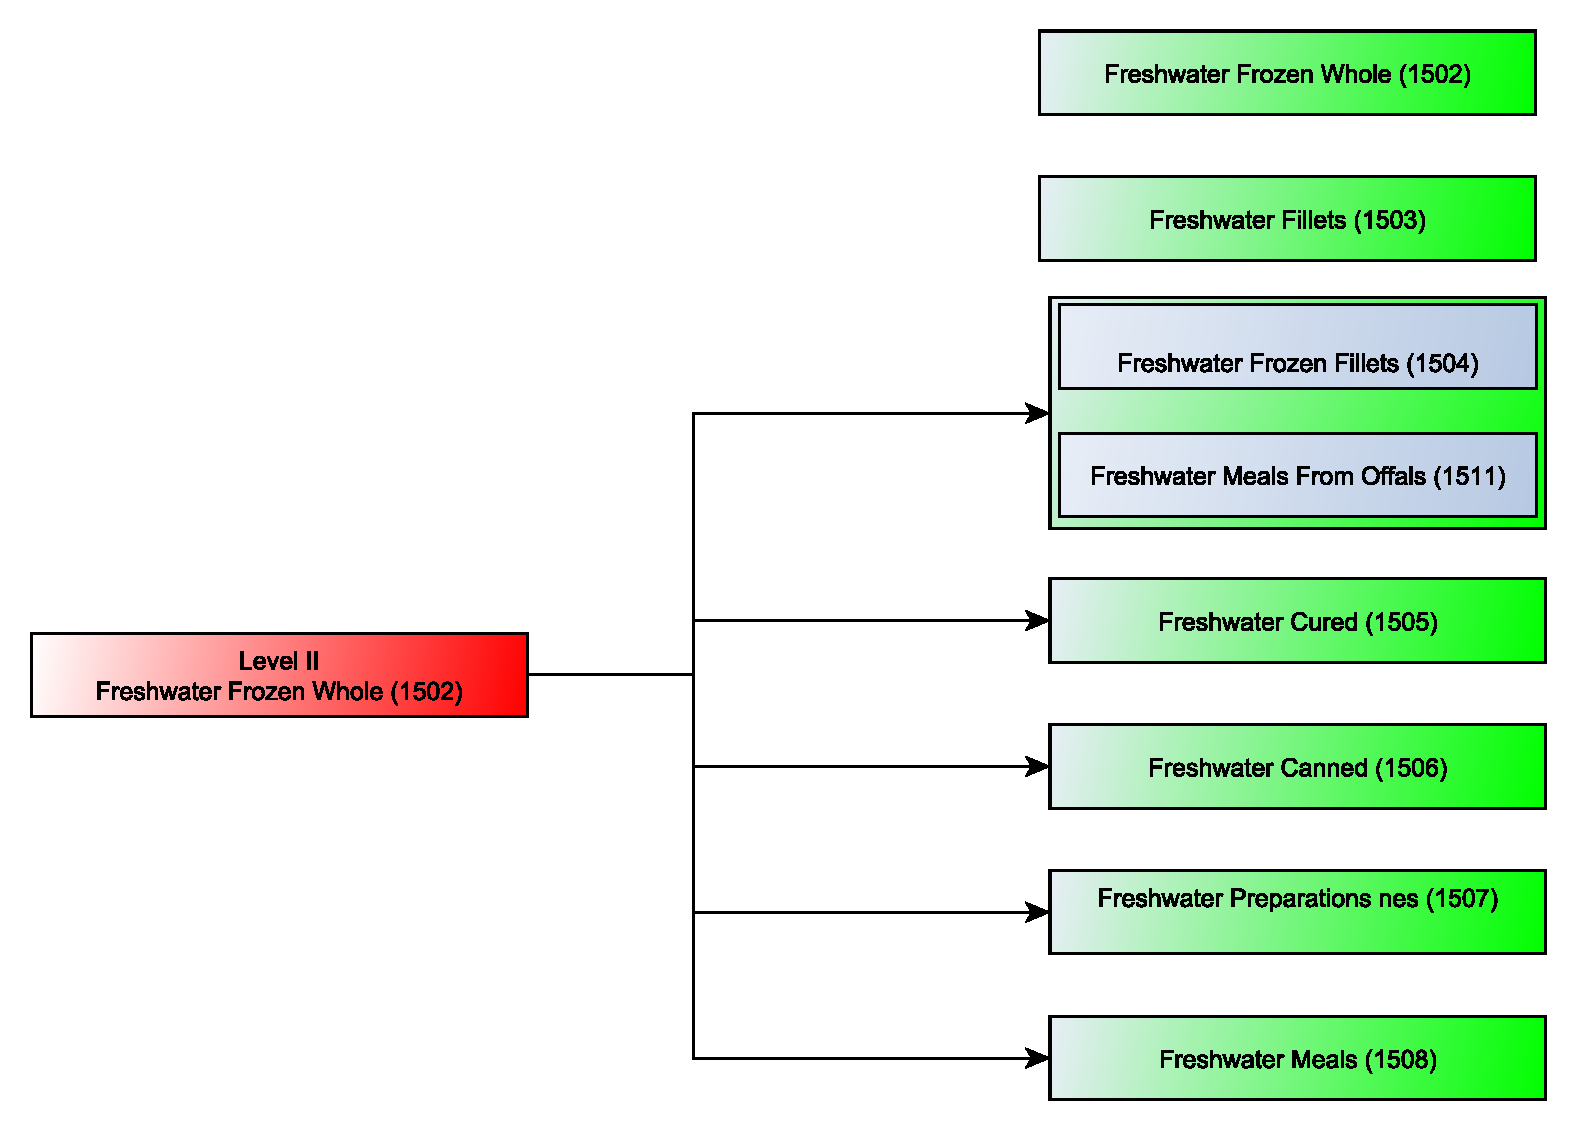
\includegraphics{flow-charts/tree/tree1502_level2.pdf}
\caption{}
\end{figure}


The commodity-tree here reported is characterized by the default extraction rates\footnotes{For R developers: according to FIAS team requirements, the extraction rates must be re-calculated if the official/protected figures are available for both \textit{production (51)} and \textit{input (31)}}. Two levels of the commodity tree are presented in the charts. This means that \textit{Freshwater Frozen Whole (1502)}, highlighted in red can be re-allocated as parent, to produce all the other by-products (1503-1508). Figure 4. and Figure 5. report only the first and second level of the commodity tree. Anyway, the set of theoretically feasible parent-child connections might be very complicated. For example: \textit{Freshwater Fillets (1503)} could be theoretically re-allocated in the processes leading to \textit{Freshwater Frozen Fillets (1504)}, \textit{Freshwater Cured (1505)}, \dots

Despite the complicated network of theoretically feasible parent-child connections, the connections actually active composing the actual commodity-trees (which are country-year specific) represents a small sub-set of all the feasible combinations. Next session is addressed to explain how the R module actives connections where the parent-commodity is not a primary item, allowing for the possibility of producing a derived product from an already processed good (but at an higher level in the supply-chain)\footnote{For R developer: the project repository contains the routine to populate the country- specific \textit{commodityTree} in the sub-folder \textit{additionalRoutines/buildTree}}. 


\subsubsection{Compute Food Processing}

The computation of the \textit{food processing} component depends on the structure of the commodity tree. The first assumption is that only primary items have been used as input to produce all the processed and preserved items\footnote{For R developpers: at the time this document has been written, the function that computes the \textit{food processing } is still under developent. Several attempts had been performed in order to reproduce an approach similar to the best-practice enstablished in FIAS department. For further details look at the functions \textit{processingComputeSimplified} and \textit{processingCompute}}. 
Assuming that only primary items can be used as input, all the connections between two derived items are cut and the resulting commodity tree\footnote{\textit{treePrimary} in the R function.} has just one level. 

As shown in Figure . the \textit{food processing} computations forsees several steps:

\begin{itemize}
\item{For all processed and preserved items the \textit{input (element 31)} is computed. Note that the \textit{input} is always expressed in terms of primary equivalent. Anyway, sometimes it may happen that the country releases official data also for the \textit{input (31)} component,  the extraction rate is thus obtained as a ratio:

$$
extractionRate_{i}= \frac{production_{i}}{input_{i}}
$$

where \textit{i} runs over the processed and preserved commodity.}

\item Once \textit{input} for all processed and preserve commodities has  been computed (actually missing), its aggregation, by parent, corresponds to the overall quantity of primary item that has been used to produce derived items. In other word it corresponds to the primary \textit{processing (131)} component.
Table 5. summarizes this procedure, it refers to the commodity tree of  \textit{ Pelagic Marine Fish Fresh (1527)}. The table shows that \textit{Pelagic Frozen Whole (1528)},   \textit{Pelagic Cured (1531)},   \textit{Pelagic Canned (1532)},   and \textit{Pelagic Meals (1534)} have been produced  using as input  \textit{ Pelagic Marine Fish Fresh (1527)} in Greece in 2013.

\begin{table}[t]
\caption{Primary Food Processing computation, data refers to Greece-2013}
\centering
\begin{tabular}{c|c|c|c|c|c}
\toprule
Primary Item & Processed Items & Production (5510) & Extraction Rate & Formula & Input (31) \\
\midrule
 
1527 &                    &               &                 &               &                  \\
     &      1528          &      985      &        0.9      &   985/0.9     &       1094.444   \\
     &      1531          &      418      &        0.4      &   418/0.4     &       1045.000   \\
     &      1532          &      3440     &        0.5      &  3440/0.5     &       6880.000   \\
     &      1534          &      200      &        0.2      &   200/0.2     &       1000.000   \\
\midrule     
     &                    &               &                 &               &        $\sum$    \\
Processing (1527)         &               &                 &               &               &    10019.44  \\  
     
\bottomrule
\end{tabular}
\label{tab:xxx}
\end{table}

\item Finally the \textit{primary processing} just computed has to be compared with the primary availability to ensure that the overall amount of available primary item ((1527) in the example), is at least enough to cover the production of all the processed and preserved items. In case the primary availability is lower than the just computed \textit{processing}, it is necessary to enlarge the set of parent items and to allow for the possibility that also a derived item can be used as input to produce by-products at a lower level in the supply-chain.

The choice of the alternative parent item to be used as input depends once again in the commodity tree. The active parent-child connections depend on the past SUA equations. 

The rationale is to keep at primary level only the amount of \textit{processed} that balance the priamary SUA equation and to deviate the exceeding quantity \footnote{Note that the amout of processed to be deviated onto an alternative parent items (which is not a primary product) has to be multiplied by the extraction rate since it has to be expressed in terms of \textit{secondary parent} equivalent.} onto an alternative parent item.

\end{itemize}




\subsection{SUA balanced table}
Once the \textit{processing} component has been properly evaluated and eventually negative unbalance checked and corrected,  those SUA equations still characterized by a positive unbalance need to be balanced. The FIAS best practice is based on the \textit{single balancer} approach: the total amount of imbalance is allocated to one component that is used as balancing element. This latter component is chosen looking at the past SUA tables. The balancing elements used in the past are country-year-item specific and they have been extrapolated (looking at the flag \textbf{B}) from the already existing SUA tables and stored in a separate table\footnote{For R developer: ''\textit{CuntryCode}-balancingElements by country are available in the project repository. The R routine to extrapolate this table is also available in the folder \textit{additionalRoutines/balancingElement.R}}.



Anyway, for many SUA equations a single balancer may not be enough to properly allocate the overall amount of availability. It is possible that a too large amount of some commodities are allocated to one single component (generally \textit{food}, \textit{feed} or \textit{other utilizations}). Here below are reported several options to overcome this issue and to split the availability to more than one SUA component:

\begin{itemize}
\item muanually impute any SUA elements (excluding the balancing element that will be automatically populated) in the \textit{SUA unbalanced} table. The user, who has observed an huge amount of availability that ends up in one single component (that does not result in line with its trend, or simply results unfeasible) can manually add another componet in the \textit{SUA unbalanced}. This operation will reduce the final availability that will be allocated to the balancing element.
\item It would be possible to build a table containing the country-year-item specific  balancing elements that allows for more than one balancing element. This solution requests to choose in advance the percentages to split the final amount of availability resulting from the SUA equation into two or more components.
\item Adapt the \textit{inverse ranking} alghoritm to the FIAS purposes\footnote{For a comprehensive discussion on the \textit{inverse ranking} alghoritm make reference to  \href{https://github.com/SWS-Methodology/faoswsFBSdocumentation/blob/master/documentation/New_Documentation_2018/02_StandDocs_Methodology.pdf}{Standardization and Balancing methodology} }. This last solution would automate the SUA balancing, but at the same time produces results that are more difficult to interpret and to modify manually.
\end{itemize}

\section{Nutritive Values and DES calculation}
After the \textit{SUA balanced} table has been produced,
\textbf{Nutritive values} are calculated: (\emph{Calories},
\emph{Proteins} and \emph{Fats}), based on the resulting Food availability
compiled after the \textit{balancing} procedure. These variables are calculated
using official Nutritive Factors
stored in the SWS. Values of Nutritive elements are stored in the system
in a datatable stored in the \textit{Fisheries} domain: \textit{fishery_nutrient}\footnote{fishery_nutrient has been provided by FIAS team, and it has been extracted from the current FIAS working system.}.


After all Nutritive Values are calculated, the Dietary Energy Supply (DES) can be compiled. DES is given by:

\begin{equation}
\label{eq:des}
 DES_{ijt} = \cfrac{\cfrac{Kcal_{ijt}}{Population_{jt}}}{365}
\end{equation}

where the \(i\) index runs over all countries, the \(j\) index over all
commodities, and \(t\) over years.



\section{FBS compilations}

The \textit{Standardization} is the process of expressing all the
processed commodities in terms of their primary equivalent and to add up all the calories of the
food commodities. One of the most important uses of the FBS consists indeed of measuring the overall average calorie supply in a country. 

The Dietary Energy Supply (DES) is not only a standard output of the FBS, but also the key input into the FAO indicator of undernourishment, i.e. the number of undernourished people and the prevalence of undernourishment. 
In addition the FBS contains a complete picture of the source of consumption on that primary item in all its forms. This procedure allows comparisons among the various processed items deriving from the same primary item, across time and countries.


Some differences occur in the way standardization is carried out according to FIAS and FAOSTAT methodologies. This difference mainly consists in the way \textit{meals} data are handled, and in taking into account both edible and inedible products (as in FAOSTAT) or only the edible component (as in FIAS). The final result of the total food fish supply and per capita food fish supply is practically identical.  

The both approaches have to be implemented and their output will be used for different dissemination purposes\footnotes{For R developper: \textit{fisheryStandardizeTree} is the function that has been developped to performe the Standardization, at the moment the focus is on the FAOSTAT methodology}.

The major differences consist in how \textit{meals} are trated. In particular, \textit{meals}\footnote{List of \textit{meal} items: Freshwater Meals (1508), Demersal Meals (1521), Pelagic Meals (1534), Marine nes Meals (1547), Crustaceans Meals (1558), Molluscs Meals (1566), Cephalopods Meals (1575), Aquatic Animals Meals (1589).} are not reported in terms of their primary equivalent according to the FIAS approach. For a comprehensive discussion of the Standardization FIAS approach, make reference to the document \href{https://unfao.sharepoint.com/:f:/s/pwa/SWS%20Phase%20III/EibKX3qrwsNAhKrHrkvTJgsBEu8Lb7NKyo5y52xl2CUXtg?e=0LuuC6}{Fiahery Standardization}: the last sections present, commodity by commodity, how to aggregate SUA equations into FBS following both FIAS and FAOSTAT approaches.

\begin{center}
\begin{figure}
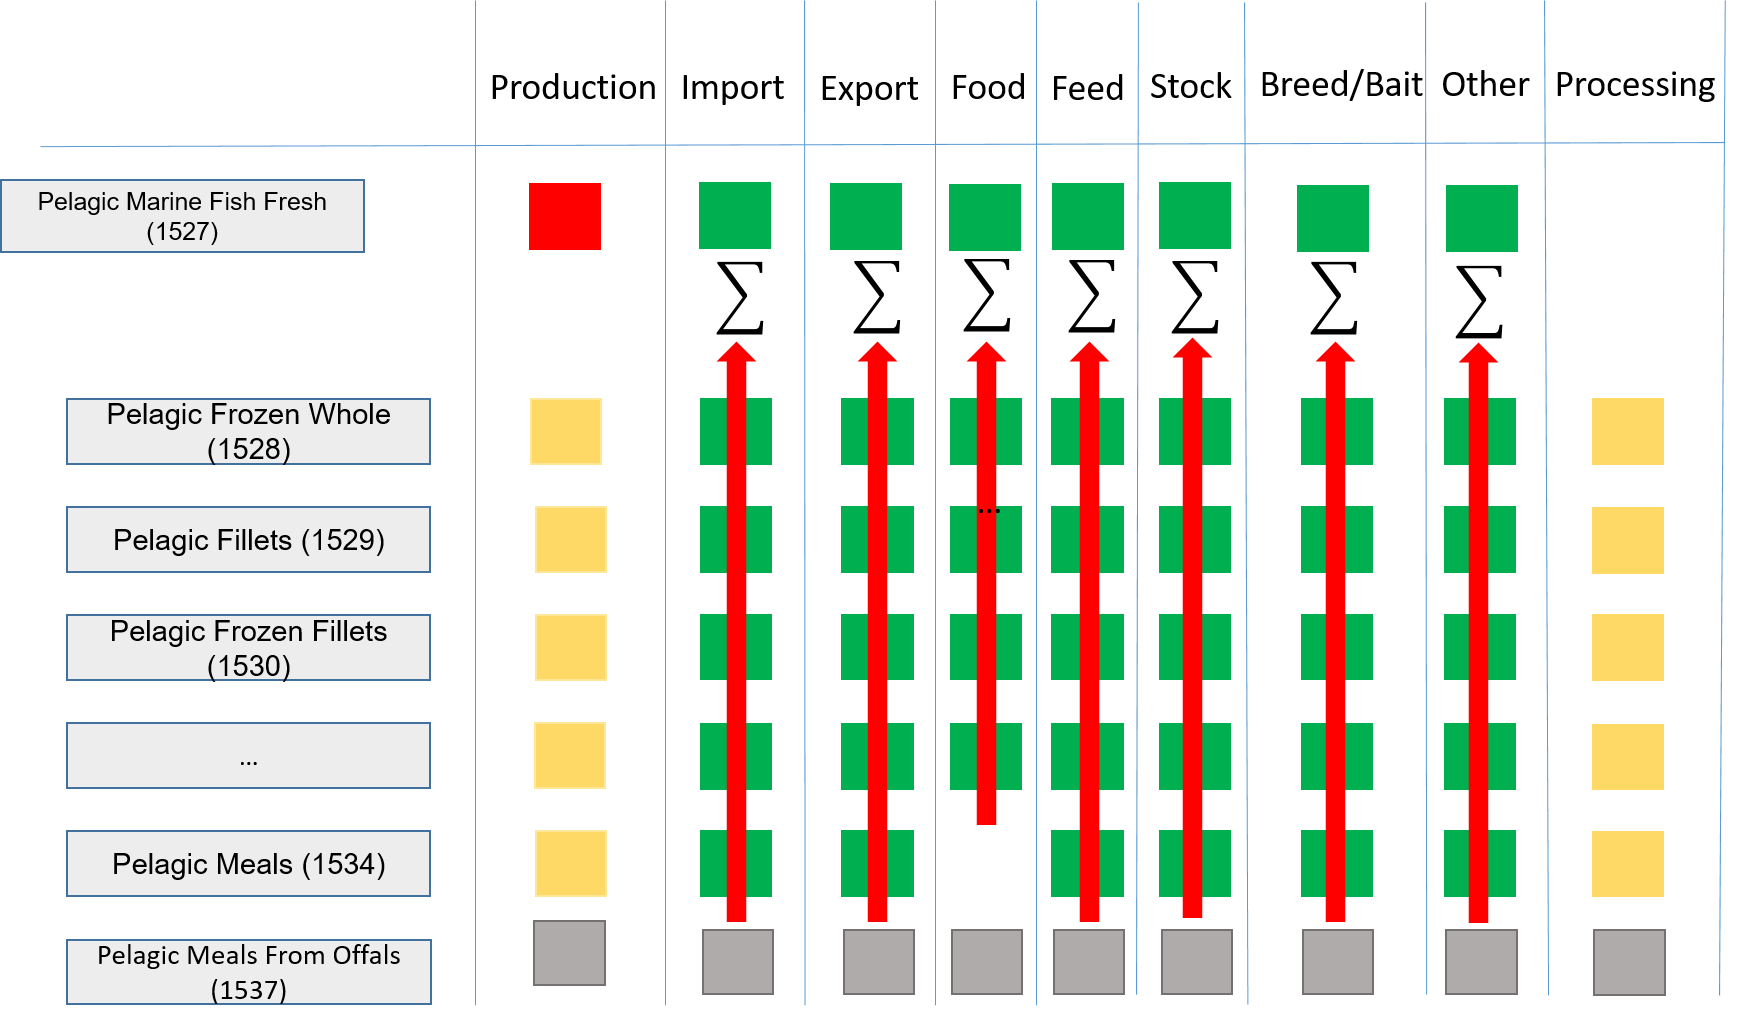
\includegraphics{flow-charts/standardization/FAOSTAT_standardization.png}
\caption{Standardization - FAOSTAT approach, example: Pelagic Marine Fish Fresh  (1527)}
\end{figure}
\end{center}


\begin{center}
\begin{figure}
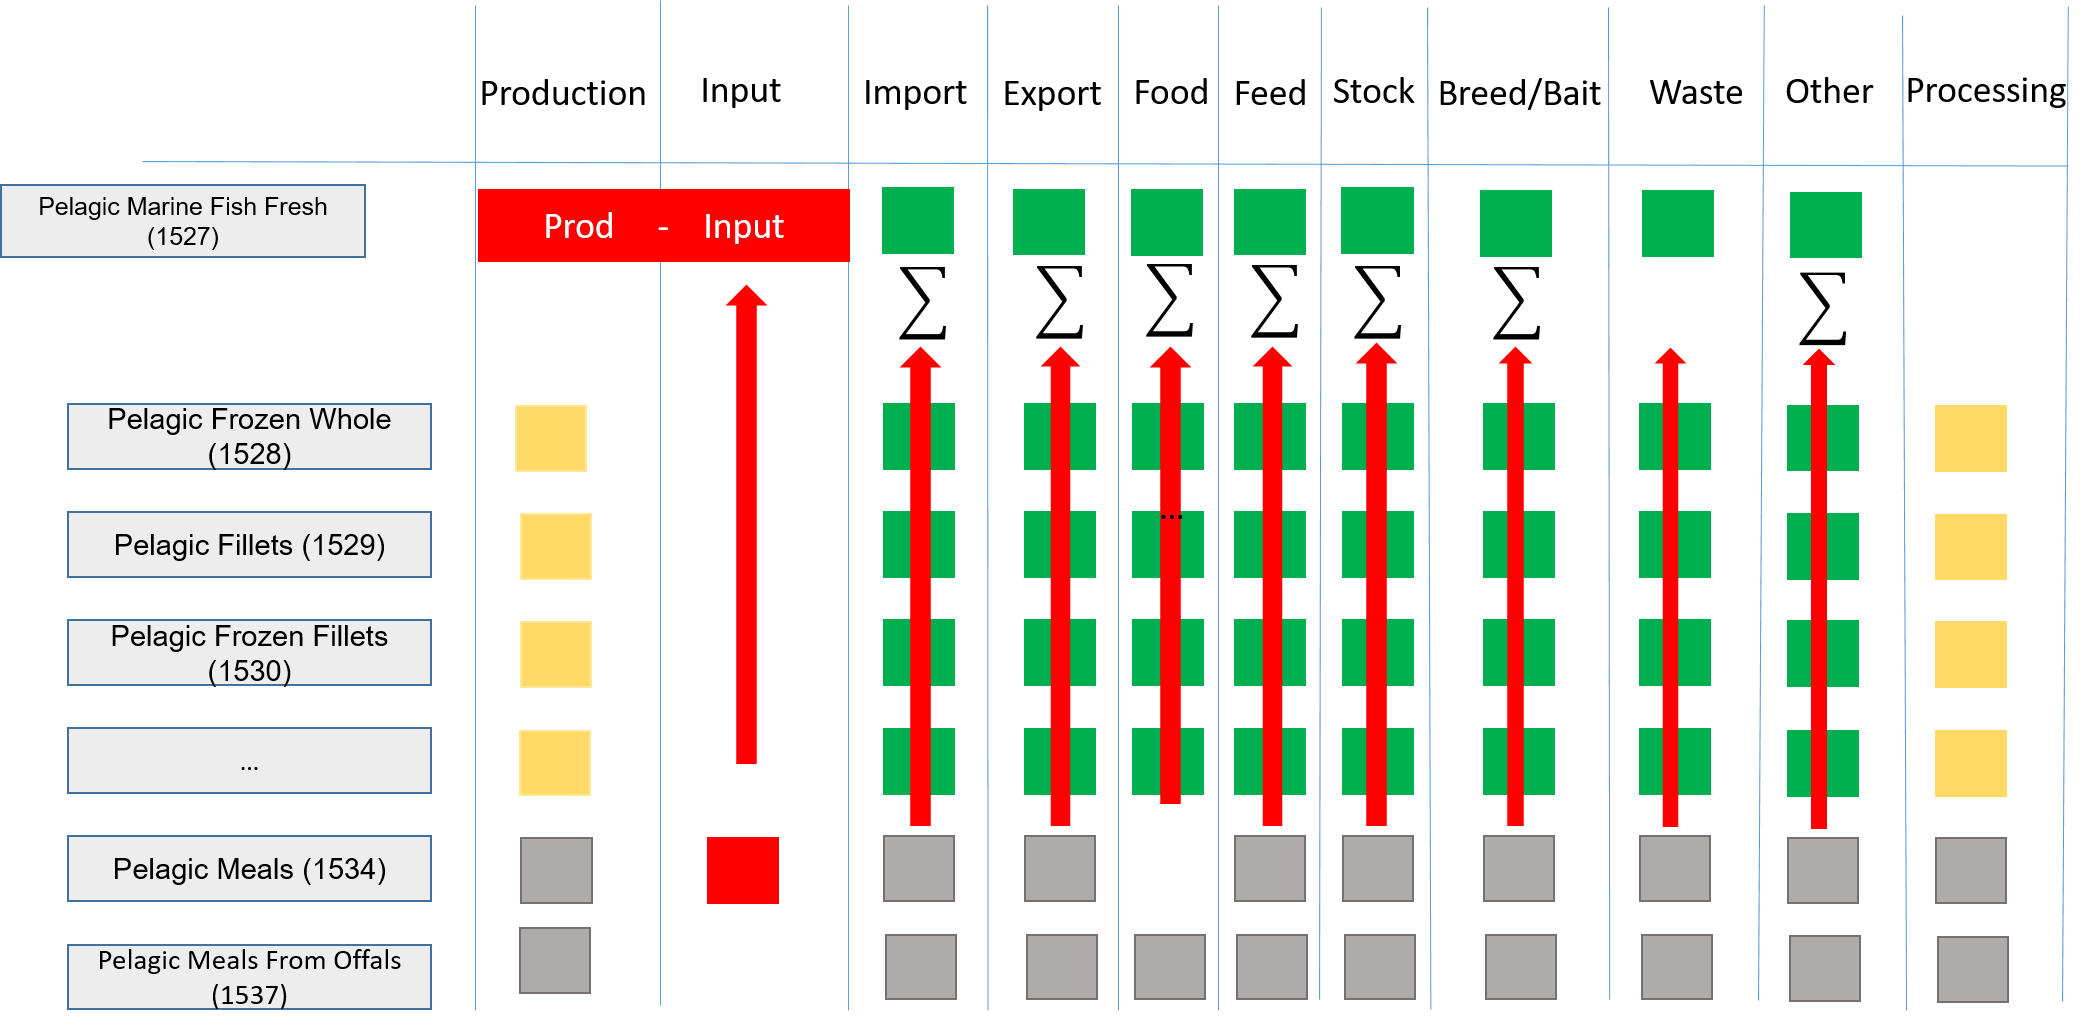
\includegraphics{flow-charts/standardization/FIAS_standardization.png}
\caption{Standardization - FIAS approach, example: Pelagic Marine Fish Fresh  (1527)}
\end{figure}
\end{center}


Finally, according to FIAS approach, the generic \textit{Other utilization} component is an aggregation of (Figure 8.):

\begin{itemize}
\item Feed;
\item Breed/Bait;
\item Waste;
\item and Other Util itsef.
\end{itemize}


\begin{center}
\begin{figure}
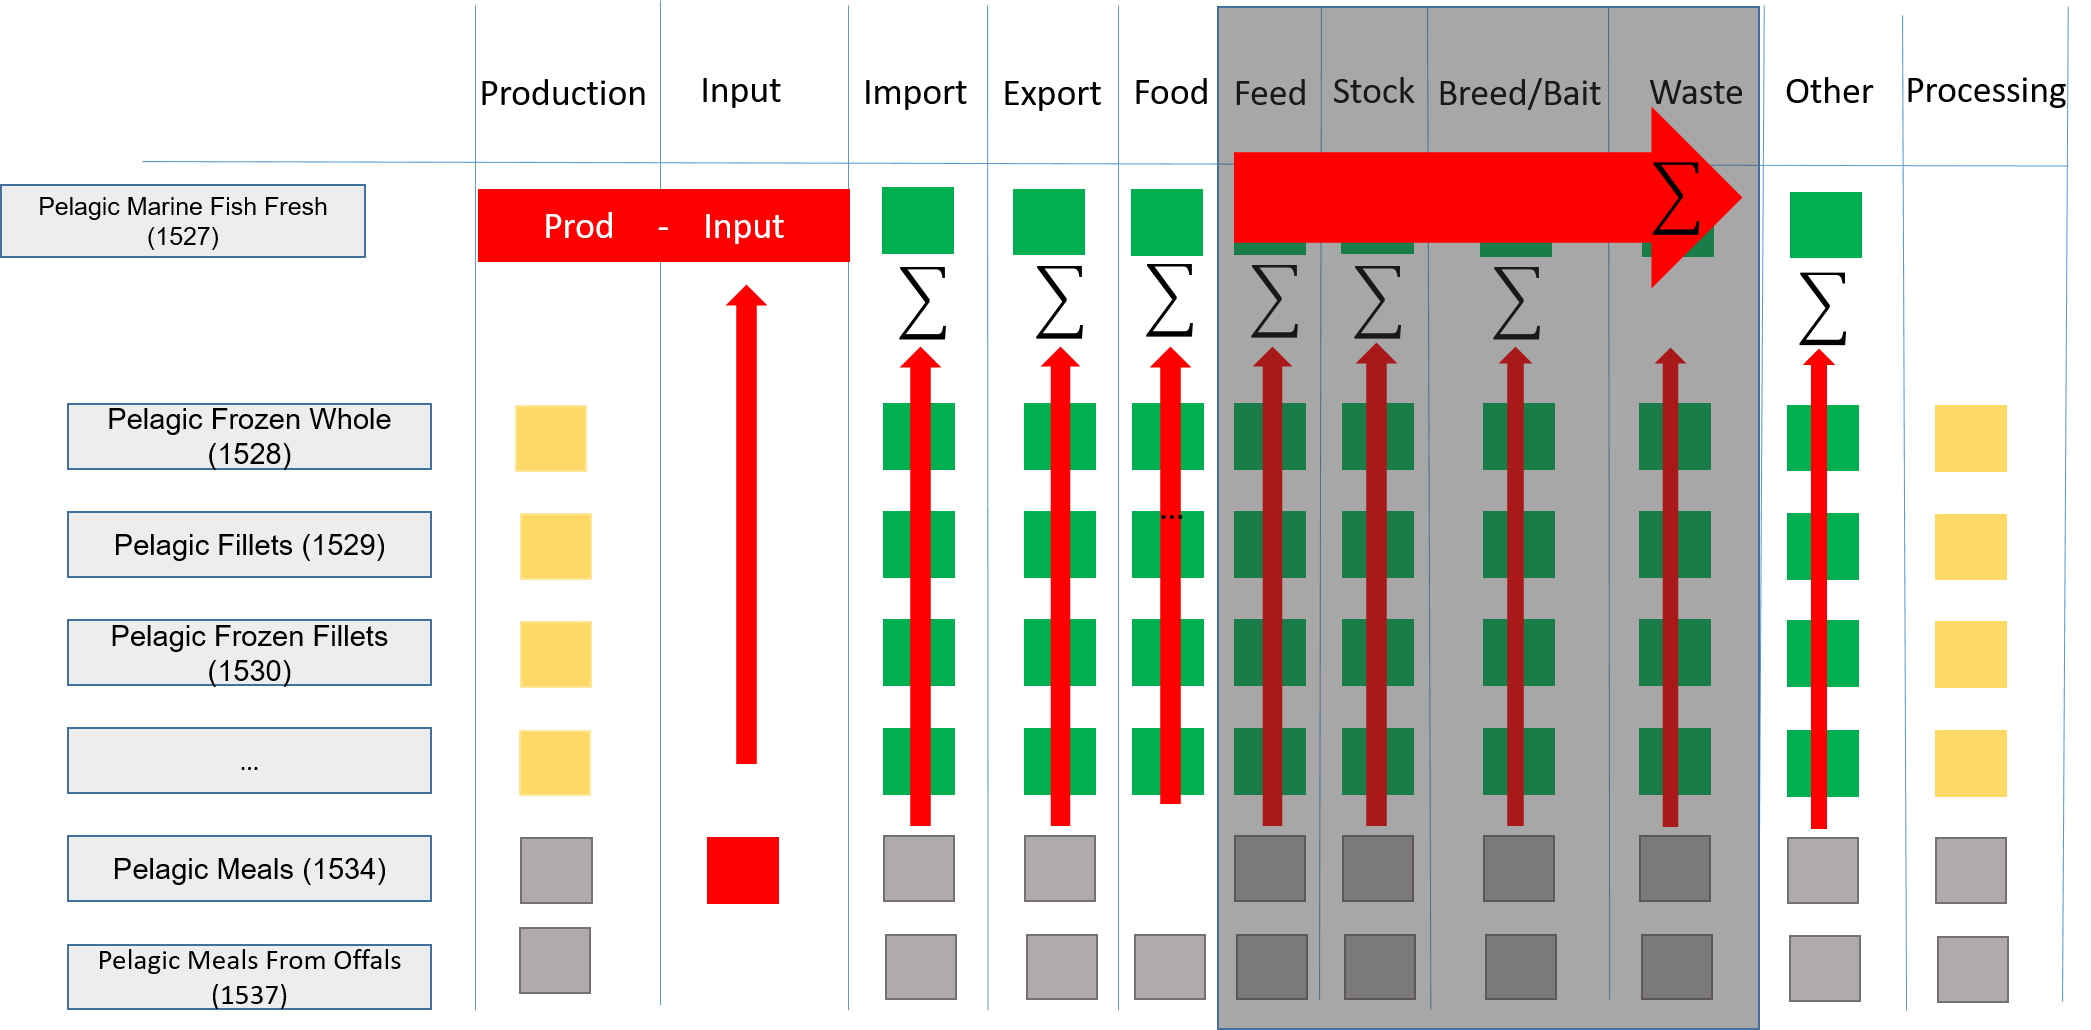
\includegraphics{flow-charts/standardization/FIAS_standardization2.png}
\caption{Standardization - FIAS approach, example: Pelagic Marine Fish Fresh  (1527). Final aggregation of Other Utilizations.}
\end{figure}
\end{center}



\end{document}
